\documentclass[12pt]{article}

% MLA format
\usepackage[letterpaper]{geometry}
\usepackage{times}
\geometry{top=1.0in, bottom=1.0in, left=1.0in, right=1.0in}
\usepackage{fancyhdr}
\pagestyle{fancy}
\lhead{} 
\chead{} 
\rhead{Simmons \thepage} 
\lfoot{} 
\cfoot{} 
\rfoot{}
\renewcommand{\headrulewidth}{0pt} 
\renewcommand{\footrulewidth}{0pt} 

\usepackage{mdwlist}
\usepackage{enumitem}
\setlist{  
  listparindent=\parindent,
  parsep=0pt,
}
\title{Homework 7}
\author{Mark Simmons}
\date{April 6, 2020}

% Multi-line glosses
%\usepackage{chngcntr}
%\usepackage{gb4e,cgloss4e}

%\newcounter{glossnum}

%\newcommand{\numgloss}{\refstepcounter{glossnum}\alph{glossnum}.\space}
%\counterwithin{glossnum}{xnumi}
%\renewcommand{\theglossnum}{\thexnumi\alph{glossnum}}

% Typing in IPA
\usepackage{tipa}

% Sentence trees
\usepackage{tikz}
\usepackage{tikz-qtree}
\usepackage{lscape}
\usepackage{graphicx}
\tikzset{level distance=30pt,
    sibling distance=6pt,
    every tree node/.style={align=center},
    }

\begin{document}

\maketitle



\begin{enumerate}[label=\textbf{\arabic*.}]
\item \textbf{Argumentation}

\item Argumentation

X-Bar theory groups types of phrases by parts of speech - noun phrase, verb phrase, adjective phrase etc. This convention is predicated on the idea that a group of words, e.g. a noun phrase, behave distributionally equivalent to a single word, e.g. a noun. A phrase by definition must have a member of its part of speech in order to be a complete phrase - a noun phrase must have a noun, and a verb phrase must have a verb. This prerequisite lexeme is known as the \emph{phrase head}.

However, we have already proposed two phrase types that do not consistently have an overt lexical head and yet are still required by the model to explain the distribution of other words and phrases in the sentence. These are TP and CP. The T and C arguments only show up overtly under certain circumstances, and yet in our analysis they are considered phrasal heads. This is in order to best explain the overall structure and distribution of the sentence as we observe it.

In this paper, I will argue that a similar reanalysis is necessary to understand the structure of NPs. Though the N argument seems the intuitive head, I propose that determiners are overall preferable candidates based on morphological structure, optionality of the N and D arguments, and distributional equivalence of the N and D arguments.

In X-Bar theory, heads are most likely to be the ``morphosyntactic locus'' of a phrase, meaning that the head is likely to mark more morphological features than any other element.

Both nouns and determiners mark the number feature to some extent.

\begin{enumerate}[label=(\arabic*)]
\item
\begin{enumerate}[label=\alph*.]
\item That dog barked.
\item Those dogs barked.
\end{enumerate}
\suspend{enumerate}


In (1a) the NP \emph{that dog} is marked for singular, and in (1b) \emph{those dogs} is marked for plural. The number morphology is expressed equally on both D and N. However, such is not always the case.

\resume{enumerate}[{[label=(\arabic*)]}]
\item
\begin{enumerate}[label=\alph*.]
\item That sheep stared at me.
\item Those sheep stared at me.
\item The dog slept.
\item The dogs slept.
\end{enumerate}
\suspend{enumerate}
It seems that the noun \emph{sheep} and the determiner \emph{the} are both invariant for number. But this is a quirk specific to these and a few other lexemes - most nouns have a distinct plural form, and most determiners either have a plural form or have in inherent and immutable number feature.
\resume{enumerate}[{[label=(\arabic*)]}]
\item
\begin{enumerate}[label=\alph*.]
\item I touched a/each/every wire!
\item *I touched a/each/every wires!
\item I touched some/several/certain wires!
\item *I touched some/several/certain wire!
\end{enumerate}
\suspend{enumerate}

Determiners such as \emph{a}, \emph{each} and \emph{every} are inherently singular; (3b) indicates that they cannot co-occur with a plural N. Likewise, \emph{some}, \emph{several} and \emph{certain} are inherently plural; they cannot co-occur with a singular N. Thus, determiners are clearly morphologically marked for number (except for \emph{the}), but most determiners do not productively inflect for both features.

Determiners are also marked for various morphological features that do not manifest on nouns, such as definiteness and deixis.

\resume{enumerate}[{[label=(\arabic*)]}]
\item
\begin{enumerate}[label=\alph*.]
\item This/that dog barked.
\item These/those dogs barked.
\item I touched the/a wire!
\item I touched the/some wires!
\end{enumerate}
\suspend{enumerate}

Sentences (4a,b) demonstrate the contrast between the proximal determiners \emph{this} and \emph{these} with distal \emph{that} and \emph{those}. (4c,d) likewise demonstrate the contrast between definite \emph{the} and indefinite \emph{a}, \emph{some} (the determiner \emph{some} is more precisely defined as paucal, but in some sentences it can mark indefiniteness, as it does in 4d).

Pronouns, which in our model are categorized with determiners, further inflect for case, where nouns do not.

\resume{enumerate}[{[label=(\arabic*)]}]
\item
\begin{enumerate}[label=\alph*.]
\item She saw the man.
\item The man saw her.
\end{enumerate}
\suspend{enumerate}

In (5a) the pronoun \emph{she} is inflected for nominative case, whereas in (5b) \emph{her} is inflected for accusative.  Nouns, on the other hand, are invariant for case - \emph{man} appears in the same form in nominative and accusative positions.

Thus, the data show that determiners have the capacity to inflect for various morphological features, whereas nouns are only capable of distinguishing number. It is thus preferable to consider that determiners are the morphosyntactic locus of their phrase, rather than nouns.

Heads are also expected to morphologically govern the rest of the phrase, requiring other elements to manifest in certain morphological forms. As discussed above, determiners and nouns agree in the number feature alone, with other features belonging solely to the determiner.

However, it bears repetition that most determiners are \emph{inherently marked} for number. The only exceptions are \emph{the}, which is unmarked, and \emph{that/those} and \emph{this/these}, which can mark for either singular or plural.

\resume{enumerate}[{[label=(\arabic*)]}]
\item
\begin{enumerate}[label=\alph*.]
\item I touched this/the/a/no/every wire!
\item I touched these/the/some/several/certain wires!
\end{enumerate}
\suspend{enumerate}

It is possible that determiners such as \emph{every} assign the [+singular] feature to the noun \emph{wire}. There is no way for the noun to assign [+singular] to \emph{every} since there is no plural form of the word \emph{every}. The definite article \emph{the} and demonstrative determiners \emph{that} and \emph{this} could then just be irregularities that appear not to assert any number feature on the noun.

In addition to morphology, a phrase head is also expected to govern optionality of its elements. The data here appear to conflict - both D and N can be missing from the NP, making it unclear as to which element governs the other.

\resume{enumerate}[{[label=(\arabic*)]}]
\item
\begin{enumerate}[label=\alph*.]
\item I touched those/these/some wires!
\item I touched those/these/some! (N is optional)
\item Those/the dogs sleep.
\item Dogs sleep. (D is optional)
\end{enumerate}
\suspend{enumerate}

Furthermore, certain Ns forbid a D argument, and certain Ds forbid an N argument.

\resume{enumerate}[{[label=(\arabic*)]}]
\item
\begin{enumerate}[label=\alph*.]
\item He pet the dog.
\item *He man pet the dog. (N is forbidden)
\item John studies syntax.
\item *The/a/every/each John studies syntax. (D is forbidden)
\end{enumerate}
\suspend{enumerate}

It appears that, with regards to optionality, the data do not seem to favor either D or N as the governing head. However, more investigation is needed. Certain groups of nouns also prevent D arguments, but I will demonstrate that this cannot be a product of syntactic government, but is due to other contextual factors.

Two groups of nouns in particular seem to exclude certain D arguments. Personal names, such as \emph{John} in (8c,d), do not appear to accept any D in the phrase. Abstract nouns such as \emph{happiness} and \emph{love} prevent some D arguments but allow others.

\resume{enumerate}[{[label=(\arabic*)]}]
\item
\begin{enumerate}[label=\alph*.]
\item Everyone wants (some/more/a lot of) happiness/love in their life.
\item *Everyone wants the/a happiness/love in their life.
\end{enumerate}
\suspend{enumerate}

It appears that the word happiness specifically forbids determiners pertaining to definiteness (\emph{the} and \emph{a}). Even then, however, there are instances where such words can appear with a definite article.

\resume{enumerate}[{[label=(\arabic*)]}]
\item
\begin{enumerate}[label=\alph*.]
\item \textbf{The happiness} of being with friends is incomparable.
\item \textbf{The love} of a mother is unconditional.
\end{enumerate}
\suspend{enumerate}

But the \emph{happiness} and \emph{love} in (10) are different from those in (9). In (10) the words to not refer to a general concept but rather a specific instantiation of the broader concept, and it is precisely this semantic structure that allows for an overt determiner which marks definiteness.

The same is even true of personal names.

\resume{enumerate}[{[label=(\arabic*)]}]
\item
\begin{enumerate}[label=\alph*.]
\item Do you know anyone named Bob?
\item \quad - Yeah. Funnily enough, all \textbf{the Bobs} I know work in construction.
\end{enumerate}
\suspend{enumerate}

Here the personal name \emph{Bob} can take a definite article when it refers a group of people who share the name \emph{Bob} rather than to a unique individual. It is possible, however, that the plural suffix \emph{-s} changes the morphology of the noun in such a way that it now allows for the definite article. In other words, \emph{Bob} and \emph{Bobs} have different distribution relative to D because of different morphological features, and not purely due to semantic context. This does not explain, however, why \emph{happiness} or \emph{love} can only take articles in contexts such as those in (10) and not others, since the morphology of these words is the same in both (9) and (10). It is more parsimonious to assume that personal names like \emph{Bob} behave similarly to abstract nouns like \emph{happiness} and \emph{love} with regards to their patterning with determiners.

Thus, it appears that proper and abstract nouns prevent determiners for semantic rather than morphological reasons. A personal name like \emph{Bob} and an abstract noun like \emph{happiness} refer to a unique entity, not a member of a set. It is only in specific instances where the referent is construed as being a member of a set (a certain type of happiness as opposed to other types of happiness, or multiple people named Bob) that definite determiners show up.


Additionally, let us consider instances where the D argument is optional.

\resume{enumerate}[{[label=(\arabic*)]}]
\item
\begin{enumerate}[label=\alph*.]
\item Dogs sleep.
\item Kids play.
\item Fish swim.
\end{enumerate}
\suspend{enumerate}

For each of the sentences in (12), the NP is grammatically plural and semantically indefinite. Making the nouns singular would render the sentences ungrammatical unless a determiner such as the indefinite article \emph{a} was present.

\resume{enumerate}[{[label=(\arabic*)]}]
\item
\begin{enumerate}[label=\alph*.]
\item *Dog sleeps.
\item A dog sleeps.
\item *Kid plays.
\item A kid plays.
\item *Fish swims.
\item A fish swims.
\end{enumerate}
\suspend{enumerate}

Again, the restriction is semantic - only when an N is indefinite and plural can it occur with no determiner. Where D forbids an N argument, however, the pattern is paradigmatic.

\resume{enumerate}[{[label=(\arabic*)]}]
\item
\begin{enumerate}[label=\alph*.]
\item *I person read.
\item *You person read.
\item *He/she person read.
\item We people read.
\item You people read.
\item \%They people read.
\end{enumerate}
\suspend{enumerate}

In most standard dialects of English, only the pronouns \emph{we} and \emph{you} (specifically when plural) can occur alongside an N (as far as the author is aware, some dialects may allow for \emph{they} to behave in the same way). This relationship is paradigmatic rather than semantic - there is no instance where the context of the phrase allows an NP such as *\emph{I person} to be grammatical.

Features of optionality (whether N is permissible, required or forbidden) are inherent (and not contingent on semantic context) for other determiners as well.

\resume{enumerate}[{[label=(\arabic*)]}]
\item
\begin{enumerate}[label=\roman*.]
\item I touched those/these/some wires!
\item I touched those/these/some!
\item I touched the/a/every wire!
\item *I touched the/a/no/every!
\end{enumerate}
\suspend{enumerate}

That \emph{the}, \emph{a}, \emph{no} and \emph{every} require an N to be complete is an inherent feature of the word - there is no context that allows any of these to function as a full grammatical phrase on their own. Similarly, \emph{those}, \emph{these}, and \emph{some} are inherently able to both co-exist in a phrase alongside an N and be the distributional equivalent of an entire phrase.

Thus, in terms of morphology, we observe three different behaviors among determiners with regard to optionality of N:

\resume{enumerate}[{[label=(\arabic*)]}]
\item
\begin{enumerate}[label=\roman*.]
\item Determiners that require a noun in the phrase (e.g. the, a, every)
\item Determiners that forbid a noun in the phrase (e.g. he, she, I)
\item Determiners that can occur with a noun in the phrase or without one (e.g. that, some, you)
\end{enumerate}
\suspend{enumerate}

While nouns also show differential behavior regarding whether they allow an accompanying D, that is the product of semantic factors, and is not due to their morphology. Determiners are inherent and immutable in deciding whether they require, allow or forbid an accompanying N argument.

Compare this to T arguments. The T \emph{will}, for example, always requires the V it immediately governs to be inflected in the bare infinitive and permits no other form, while the T \emph{be} requires the V to be in a present or past participle form. Each governing element consistently allows only a certain form or subset of forms to characterize the phrase it governs, and what forms it allows is a feature inherent to each unique governing element. This parallel between D and T arguments leads me to conclude that D arguments are the governing element in their phrase.

The issue of distributional equivalence remains. If N is not the head of its own phrase, how can it occur alone in the phrase?

\resume{enumerate}[{[label=(\arabic*)]}]
\item
\begin{enumerate}[label=\alph*.]
\item John studies syntax.
\item Love is in the air.
\item Dogs sleep.
\item Kids play.
\end{enumerate}
\suspend{enumerate}

It bears reminder that one of the features that determiners inflect for, a feature which nouns lack morphologically, is definiteness. Every noun phrase has some value for definiteness, even if it is only relevant on a pragmatic level and not marked overtly in the morphology. Thus, I propose that nouns can only occur without a determiner in the instances where information regarding definiteness can be unambiguously recovered from context. A personal name is expected to refer to a single, unique person that all participants of the conversation can identify, thus there is no need to specify whether it is definite or not. Similarly, abstract nouns refer to culturally-understood concepts, and only need to have their definiteness specified when a speaker wants to select a certain kind or instantiation of the concept.

The case of indefinite plural nouns is a bit trickier (e.g. 17a,b)  English requires indefinite singular nouns to be marked with the determiner \emph{a/an}. This could be because leaving a noun in its singular form necessarily involves specifying its exact number, which is antagonistic to the idea of indefiniteness, making [-definite -plural] more marked than [-definite +plural], where the exact number of the entity is left ambiguous. In other words, a group of referents whose number is unspecified is more likely to be indefinite, thus English leaves the article out because the indefinite reading can easily be inferred.

Based on this evidence, I posit a null determiner which is unspecified for number and definiteness, $\emptyset_{[\pm plural \pm definite]}$, which is the head of a determiner phrase (DP) in instances where the referent's definiteness is easily recoverable from context. I propose that this is a preferable alternative to assuming that nouns select for their determiner based on semantic context, since the relevant contexts primarily concern definiteness, which is a feature inflected on determiners rather than nouns. Again, this is similar to an analytical move proposed for TPs, where the T argument is sometimes a null affix that supplies the verbs tense morphology, even though it does not surface as an overt argument in T position.

The similarity of form between D and T extends beyond morphology and into their tree structure.

\resume{enumerate}[{[label=(\arabic*)]}]
\item
{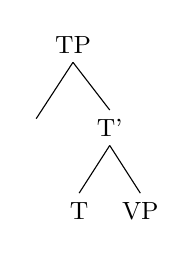
\begin{tikzpicture}
{\small \Tree
[.TP {}
	[.T' T VP ]
]
}
\end{tikzpicture}}
{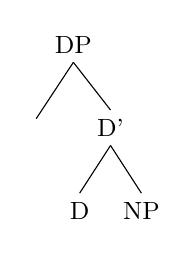
\begin{tikzpicture}
{\small \Tree
[.DP {}
	[.D' D NP ]
]
}
\end{tikzpicture}}
\end{enumerate}

This is another advantage of the proposed analysis - it unifies the trees of formally disparate phrase structures.

In summary, I propose that in order to fit the understanding of phrase heads that X-Bar provides, we must  the D argument of the NP as head rather than N. I argue this from morphological evidence - D marks far more morphological features than N does. Furthermore, where it may seem that D and N are equally capable of conditioning or preventing each other's presence, I suggest that it is preferable to assume that government flows from D rather than from N, and that instances with no overt D can be explained by a phonologically null determiner which unifies the disparate contexts where N seemingly occurs alone.

Though it may still violate human intuition to propose that D is head over N, I argue that the structure of X-Bar, particularly the parallel structure proposed for TP, requires that D be head over N in order to explain the morphological and syntactic patterns we observe.\bigskip

\noindent \textbf{Response to Comments:}
Everyone who commented on my argument very consistently pointed out its one-sidedness. Looking back, for some reason the counter arguments that had occurred to me while writing seemed genuinely not worth including at the time, like personal names for instance. Once I included them in my analysis, though, I feel my argument gained a great deal of nuance and rigor, which I owe to the constructive criticism I've received. It also made my argument twice as long, so I am genuinely sorry for making y'all slug through all six of those pages. I also received several comments suggesting I break my data up more, which, funnily enough, made it easier to construct my argument as I was writing.\bigskip

\noindent \textbf{Peer Review:}
I was pretty pleased with this process. It was really helpful to get comments from people who were unfamiliar with the prompt I was addressing, it helped me understand where my paper was not self-contained. The classmates in my peer review group never made any communication apart from commenting on each other's paper - but I personally understood all the comments I received, so it probably wouldn't have been necessary.

\item \textbf{X' Trees}

\begin{enumerate}[label=(\alph*)]
\item \leavevmode\vadjust{\vspace{-\baselineskip}}\newline
%\begin{landscape}
\noindent\resizebox{\textwidth}{!}{\begin{tikzpicture}
{\small \Tree
[.CP {}
[.C' C\\$\emptyset$
[.TP [.DP [.DP {} [.D' {} [.NP {} [.N' N\\Mary {} ] ] ] ]%N', NP, D', DP
	[.D' D\\'s [.NP {} [.N' [.AdjP {} [.Adj' Adj\\younger {} ] ]
	[.N' N\\sister {} ] ]%N', N'
	] ] ]%NP, D' DP
[.T' T\\$\emptyset$
	[.VP {} [.V' V\\put
		[.DP {} [.D' D\\the [.NP {} [.N' N\\books {} ] ] ] ]%N', NP, D', DP
		[.PP \edge[roof]; {on the shelf..} ]
	]%V'
	]%VP
]%T'
]%TP
]%C'
]%CP
}

\end{tikzpicture}}

\noindent{\begin{tikzpicture}
{\small \Tree
[.PP {} [.P' P\\on
[.DP {}
[.D' D\\the [.NP {} [.N' N\\shelf
	[.PP {} [.P' P\\on
	[.DP {} [.D' D\\the 
		[.NP {} [.N' N\\balcony {} ] ]%N', NP
	] ]%D', DP
	]%P'
	]%PP
] ]%N', NP
]%D'
]%DP
]%P'
]%PP
}
\end{tikzpicture}}

\item \leavevmode\vadjust{\vspace{-\baselineskip}}\newline
\noindent\resizebox{\textwidth}{!}{\begin{tikzpicture}
{\small \Tree
[.CP {}
[.C' C\\$\emptyset$
[.TP
	[.CP {}
	[.C' C\\That
	[.TP [.ConjP [.DP {}
		[.D' D\\$\emptyset$ [.NP {}
		[.N' N\\John {} ]%N'
		] ] ]%NP, D' DP
	Conj\\and
	[.DP {}
		[.D' D\\his [.NP {} [.N'
		[.N' {} N\\friends ]%N'
		[.PP {} [.P' P\\from [.DP {}
			[.D' D\\$\emptyset$ [.NP {}
		[.N' N\\school {} ]%N'
		] ] ]%NP, D' DP
		] ] ]%P', PP, N'
		] ] ]%NP, D' DP
	]%ConjP
	[.T' T\\$\emptyset$
		[.VP {} [.V'
			[.V' left {} ]%V'
			[.AdvP {} [.Adv' {} Adv\\early ] ]%Adv', AdvP
		]%V'
		]%VP
	]%T'
	]%TP
	]%C'
	]%CP
[.T' \edge[roof]; {means that...}
]%T'
]%TP
]%C'
]%CP
}
\end{tikzpicture}}

\noindent\resizebox{\textwidth}{!}{\begin{tikzpicture}
{\small \Tree
[.T' {}
[.VP
[.V' V\\means
	[.CP {} 
	[.C' C\\that
	[.TP [.DP {} [.D' D\\they {} ] ]%D', DP
	[.T' T\\will
		[.VP 
			[.V' V\\come [.PP {} [.P' P\\to [.DP {} [.D' D\\$\emptyset$ [.NP {} [.N' N\\work {} ] ] ] ] ] ]%N', NP, D', DP, P', PP
			]%V'
			[.PP {} [.P' P\\on [.DP {} [.D' D\\$\emptyset$ [.NP {} [.N' N\\time {} ] ] ] ] ] ]%N', NP, D', DP, P', PP
		]%VP
	]%T'
	]%TP
	]%C'
	]%CP
]%V'
]%VP
]%T'
}
\end{tikzpicture}}

\item \leavevmode\vadjust{\vspace{-\baselineskip}}\newline
%\begin{landscape}
\noindent\resizebox{\textwidth}{!}{\begin{tikzpicture}
{\small \Tree
[.CP {}
[.C' C\\$\emptyset$
[.TP
	[.DP {}
	[.D' D\\My [.NP {} [.N' [.AdjP {} [.Adj' Adj\\kind, {} ] ]%Adj', AdjP
	[.N' [.AdjP {} [.Adj' Adj\\elderly {} ] ]%Adj', AdjP
	[.N' N\\neighbour {} ] ]%N', N'
	] ] ] ]%N', NP, D' DP
[.T' T\\should
	[.VP {} [.V' V\\expect
		[.CP \edge[roof]; {that we will...}
		]%CP
	]%V'
	]%VP
]%T'
]%TP
]%C'
]%CP
}
\end{tikzpicture}}

{\begin{tikzpicture}
{\small \Tree
[.CP {}
[.C' C\\that
[.TP
	[.DP {} [.D' D\\we {} ] ]%D', DP
	[.T' T\\will
	[.VP {}
	[.V' V\\return [.DP {} [.D' D\\his [.NP {} [.N' N\\tools. {} ] ] ] ]%N', NP, D', DP
	]%V'
	]%VP
	]%T'
]%TP
]%C'
]%CP
}
\end{tikzpicture}}

\item \leavevmode\vadjust{\vspace{-\baselineskip}}\newline
{\begin{tikzpicture}
\tikzset{every tree node/.style={align=center,anchor=north}}
{\small \Tree
[.CP {}
[.C' C\\$\emptyset$
[.TP
	[.CP {}
	[.C' C\\For
	[.TP
		[.DP {} [.D' D\\you {} ] ]%D', DP
		[.T' T\\to
		[.VP {}
		[.V' V\\{stay up} {}
		]%V'
		]%VP
		]%T'
	]%TP
	]%C'
	]%CP
[.T' \node(t){T\\-s$_{[+pres]}$};
	[.VP {}
	[.V' \node(v){V\\impress}; [.DP {} [.D' D\\me. {} ] ]%D', DP
	]%V'
	]%VP
]%T'
]%TP
]%C'
]%CP

\draw[semithick,->] (t)..controls +(south west:2) and +(south west:4)..(v);
}
\end{tikzpicture}}

\end{enumerate}

% theta bois
\pagebreak
\item \textbf{Theta Grids}

\begin{enumerate}[label=(\arabic*)]
\item
\begin{enumerate}[label=\alph*.]
\item Ken$_{i}$ left the book$_{j}$.\\
\begin{tabular}{ |c|c|c| } 
 \hline
 \underline{agent} & patient & location \\ 
 DP & DP & (PP) \\ 
 \hline
 i & j & \\ 
 \hline
\end{tabular}
\item Ken$_{i}$ left the book$_{j}$ on the shelf$_{k}$.\\
\begin{tabular}{ |c|c|c| } 
 \hline
 \underline{agent} & patient & location \\ 
 DP & DP & (PP) \\ 
 \hline
 i & j & k \\ 
 \hline
\end{tabular}
\item John$_{i}$ mailed a letter$_{j}$.\\
\begin{tabular}{ |c|c|c| } 
 \hline
 \underline{agent} & patient & recipient \\ 
 DP & DP & (PP) \\ 
 \hline
 i & j &  \\ 
 \hline
\end{tabular}
\item John$_{i}$ mailed a letter$_{j}$ to Sandy$_{k}$.\\
\begin{tabular}{ |c|c|c| } 
 \hline
 \underline{agent} & patient & recipient \\ 
 DP & DP & (PP) \\ 
 \hline
 i & j & k \\ 
 \hline
\end{tabular}
\item John$_{i}$  mailed Sandy$_{j}$ a letter$_{k}$.\\
\begin{tabular}{ |c|c|c| } 
 \hline
 \underline{agent} & recipient & patient \\ 
 DP & DP & DP \\ 
 \hline
 i & j &  \\ 
 \hline
\end{tabular}
\item Kim$_{i}$ shattered the vase $_{j}$.\\
\begin{tabular}{ |c|c| } 
 \hline
 \underline{agent} & patient \\ 
 DP & DP \\ 
 \hline
 i & j \\ 
 \hline
\end{tabular}
\item The vase$_{i}$ shattered.\\
\begin{tabular}{ |c| } 
 \hline
 \underline{patient} \\ 
 DP \\ 
 \hline
 i \\ 
 \hline
\end{tabular}
\end{enumerate}
\item
\begin{enumerate}[label=\alph*.]
\item The verb \emph{leave} c-selects a PP for the Theta-role of location, not a DP.
\item The verb \emph{leave} c-selects a DP for the Theta-role of patient. This argument cannot be omitted.
\item The transitive verb \emph{shatter} c-selects a patient DP which this sentence lacks. The intransitive sense of the verb s-selects an intransitive, solid object as its subject (which has the Theta-role of experiencer), thus it \emph{Ken} is not a valid DP for the role.
\item The ditransitive verb \emph{mail} c-selects one DP as the recipient and one DP as the patient, no more DPs are allowed as complements to the verb.
\item The ditransitive verb \emph{mail} c-selects a DP as the patient following the DP expressing the recipient argument. The monotransitive verb \emph{mail} s-selects an inanimate object for the patient argument, thus \emph{Sandy} is not a valid DP for the role.
\end{enumerate}
\end{enumerate}

\pagebreak
\item \textbf{Sinhala}
\begin{enumerate}[label=(\arabic*)]
\item
\begin{enumerate}[label=\alph*.]
\item Siri$_{i}$ kawi$_{j}$ ki\textipa{@}n\textipa{@}wa.\\
\begin{tabular}{ |c|c| } 
 \hline
 \underline{agent} & patient \\ 
 DP & DP \\ 
 \hline
 i & j \\ 
 \hline
\end{tabular}

\item Siri\d{t}\textipa{@}$_{i}$ kawi$_{j}$ ki\textipa{@}wen\textipa{@}wa.\\
\begin{tabular}{ |c|c| } 
 \hline
 \underline{experiencer} & patient \\ 
 DP & DP \\ 
 \hline
 i & j \\ 
 \hline
\end{tabular}


\item Lamea$_{i}$ kataaw\textipa{@}$_{j}$ ahan\textipa{@}wa.\\
\begin{tabular}{ |c|c| } 
 \hline
 \underline{agent} & patient \\ 
 DP & DP \\ 
 \hline
 i & j \\ 
 \hline
\end{tabular}

\item Lamea\d{t}\textipa{@}$_{i}$ kataaw\textipa{@}$_{j}$ \ae hen\textipa{@}wa.\\
\begin{tabular}{ |c|c| } 
 \hline
 \underline{experiencer} & patient \\ 
 DP & DP \\ 
 \hline
 i & j \\ 
 \hline
\end{tabular}

\item Siri$_{i}$  na\d{t}\textipa{@}n\textipa{@}wa.\\
\begin{tabular}{ |c| } 
 \hline
 \underline{agent} \\ 
 DP \\ 
 \hline
 i \\ 
 \hline
\end{tabular}

\item Siri\d{t}\textipa{@}$_{i}$  n\ae \d{t}en\textipa{@}wa.\\
\begin{tabular}{ |c| } 
 \hline
 \underline{experiencer} \\ 
 DP \\ 
 \hline
 i \\ 
 \hline
\end{tabular}

\item H\ae m\textipa{@} irida m\textipa{@} Nimal$_{i}$ Kol\textipa{@}mb\textipa{@}$_{j}$ yan\textipa{@}wa.\\
\begin{tabular}{ |c|c| } 
 \hline
 \underline{agent} & goal \\ 
 DP & DP \\ 
 \hline
 i & j \\ 
 \hline
\end{tabular}

\item H\ae m\textipa{@} irida m\textipa{@} Nimal\d{t}\textipa{@}$_{i}$ Kol\textipa{@}mb\textipa{@}$_{j}$ y\ae wen\textipa{@}wa.\\
\begin{tabular}{ |c|c| } 
 \hline
 \underline{experiencer} & goal \\ 
 DP & DP \\ 
 \hline
 i & j \\ 
 \hline
\end{tabular}

\item Malli$_{i}$ unt\textipa{@} $_{j}$ banin\textipa{@}wa.\\
\begin{tabular}{ |c|c| } 
 \hline
 \underline{agent} & patient \\ 
 DP & DP \\ 
 \hline
 i & j \\ 
 \hline
\end{tabular}

\item Malli\d{t}\textipa{@}$_{i}$ unt\textipa{@}$_{j}$ b\ae nen\textipa{@}wa.\\
\begin{tabular}{ |c|c| } 
 \hline
 \underline{experiencer} & patient \\ 
 DP & DP \\ 
 \hline
 i & j \\ 
 \hline
\end{tabular}
\end{enumerate}
\item Where the A-verb forms select an agent role as the subject, the P-forms select an experiencer.
\item The suffix \emph{-\d{t}\textipa{@}} attaches to DPs in the experiencer role.
\end{enumerate}

\end{enumerate}
\end{document}
